\def\mytitle{MATRICES USING PYTHON}
\def\myauthor{THOUTU RAHUL RAJ}
\def\contact{rdj4648@gmail.com}
\def\mymodule{Future Wireless Communication (FWC)}
\documentclass[10pt, a4paper]{article}
\usepackage[a4paper,outer=1.5cm,inner=1.5cm,top=1.75cm,bottom=1.5cm]{geometry}
\twocolumn
\usepackage{graphicx}
\graphicspath{{./images/}}
\usepackage[colorlinks,linkcolor={black},citecolor={blue!80!black},urlcolor={blue!80!black}]{hyperref}
\usepackage[parfill]{parskip}
\usepackage{lmodern}
\usepackage{amsmath,amsfonts,amssymb,amsthm}
\usepackage{tikz}
	\usepackage{physics}
%\documentclass[tikz, border=2mm]{standalone}
\usepackage{karnaugh-map}
%\documentclass{article}
\usepackage{tabularx}
\usepackage{circuitikz}
\usetikzlibrary{calc}
\usepackage{amsmath}
\usepackage{amssymb}
\renewcommand*\familydefault{\sfdefault}
\usepackage{watermark}
\usepackage{lipsum}
\usepackage{xcolor}
\usepackage{listings}
\usepackage{float}
\usepackage{titlesec}
\providecommand{\norm}[1]{\left\lVert#1\right\rVert}
\providecommand{\sbrak}[1]{\ensuremath{{}\left[#1\right]}}
\providecommand{\lsbrak}[1]{\ensuremath{{}\left[#1\right.}}
\providecommand{\rsbrak}[1]{\ensuremath{{}\left.#1\right]}}
\providecommand{\brak}[1]{\ensuremath{\left(#1\right)}}
\providecommand{\lbrak}[1]{\ensuremath{\left(#1\right.}}
\providecommand{\rbrak}[1]{\ensuremath{\left.#1\right)}}
\providecommand{\cbrak}[1]{\ensuremath{\left\{#1\right\}}}
\providecommand{\lcbrak}[1]{\ensuremath{\left\{#1\right.}}
\providecommand{\rcbrak}[1]{\ensuremath{\left.#1\right\}}}
\newcommand{\myvec}[1]{\ensuremath{\begin{pmatrix}#1\end{pmatrix}}}
\let\vec\mathbf
\providecommand{\mtx}[1]{\mathbf{#1}}
\titlespacing{\subsection}{1pt}{\parskip}{3pt}
\titlespacing{\subsubsection}{0pt}{\parskip}{-\parskip}
\titlespacing{\paragraph}{0pt}{\parskip}{\parskip}
\newcommand{\figuremacro}[5]

\begin{document}

\title{\mytitle}
\author{\myauthor\hspace{1em}\\\contact\\FWC22008\hspace{6.5em}IITH\hspace{0.5em}\mymodule\hspace{6em}ASSIGN-5}
\date{}
	\maketitle
		
	\tableofcontents
\vspace{5mm}
   \section{Problem}
\textbf{ Draw a circle and two lines parallel to a given line such that one is a tangent and the other is a secant to the circle }
 \section{Construction}
 	\begin{center}
     Figure of Construction
     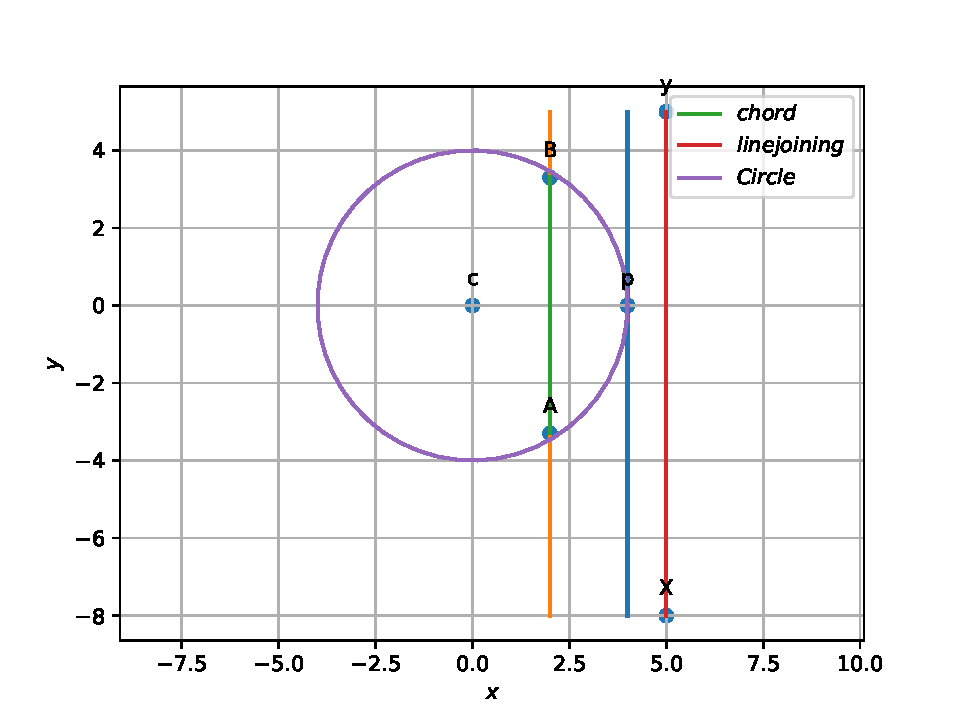
\includegraphics[scale=0.5]{figs/fig.pdf} 
  	\end{center}
  	The input parameters for this construction are 
\begin{center}
\begin{tabular}{|c|c|c|}
	\hline
	\textbf{Symbol}&\textbf{Value}&\textbf{Description}\\
	\hline
	r&4&Radius of the circle\\
	\hline		
	c&5&constant \\
	\hline
	\textbf{C}&$\
	\begin{pmatrix}
		0 \\
		0 \\
	\end{pmatrix}$
	&center\\
	\hline
	
\end{tabular}
\end{center}

   \section{Solution}

\vspace{1mm}
\textbf{Termux commands :}
\begin{lstlisting}
python3 xyz.py
\end{lstlisting}


\vspace{.25 cm}
\textbf{To Prove:}
In a given circle and a line draw two lines such that one is a secant and other one is tangent. 

 Given:
Circle center with (0,0), radius 4 and a line. \\
\begin{align}
\vec{x}^{\top}\vec{V}\vec{x}+2\vec{u}^{\top}\vec{x}+f=0
\end{align}	
$\vec{V}$ = $\begin{pmatrix}
 1 & 0\\
 0 & 1
 \end{pmatrix}$,
 $\vec{u}$=$\vec{\begin{pmatrix}0 \\0 \end{pmatrix}}$
 \textit{f = -16}\\
 By substituting above values in the equation (1) ,
 we get cirle equation.

Now let us take the given line equation as\\
\begin{align}
\vec{n}^tx=5
\end{align}
condition for tanget to the given circle will be
\begin{align}
D = \pm C\\
\vec{D}= \pm \sqrt{e^2\brak{\vec{u}^{\top}\vec{n}}^2-\lambda_2\brak{e^2-1}\brak{\norm{\vec{u}}^2 - \lambda_2 f}}
\end{align}
by sloving the above eq we get,
\begin{align}
D = \pm 4 
\end{align}

and the condition for secant which is also parallel to the given line will be
\begin{align}
D \geq 0 
\end{align}
i.e 
\begin{align}
-4 < C < 4
\end{align}
\vspace{1mm}
The below python code realizes the above construction:	\\
\url{https://github.com/Rahulraj00/Assignments/tree/main/Assignments/assg_5/xyz.py}
\bibliographystyle{ieeetr}
\end{document}
